\section{Properties of Pure Substances}\label{sec:Properties_Pure_Substances}
Many of the substances that we study in \nameref{def:Thermodynamics} are what we call \nameref{def:Pure_Substance}s.

\begin{definition}[Pure Substance]\label{def:Pure_Substance}
  A \emph{pure substance} is one whose chemical composition is fixed throughout.
  Properties of these substances are completely known, and these properties are completely uniform throughout the substance.
\end{definition}

In general, the pressure of a substance is an exponential function that is dependent on the temperature of the water.
In addition, the pressure of the substance depends on its altitude.
As you increase in altitude, this means that the temperature required to boil the substance at decreases.
All of these are visualized in \Cref{fig:Temp_Pressure_Liquid_Vapor_Curve}.

\begin{figure}[h!tbp]
  \centering
  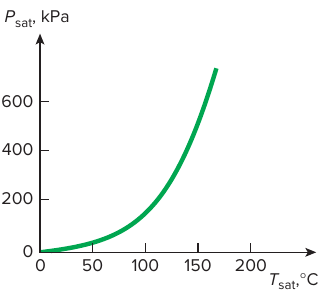
\includegraphics[scale=0.75]{./Temperature_Pressure_Liquid_Vapor_Curve.png}
  \caption{Temperature-Pressure ($\Temp$-$\Pressure$) Liquid-Vapor Curve}
  \label{fig:Temp_Pressure_Liquid_Vapor_Curve}
\end{figure}

\subsection{Phase Changes}\label{subsec:Phase_Changes}
Phase changes in materials are unique, because they maintain a constant temperature \textbf{until} all the material undergoes the phase change, however, the volume increases \textbf{drastically}.

\begin{definition}[Phase Change]\label{def:Phase_Change}
  A \emph{phase change} in a substance is when it changes from one state of matter to another.
  This means a substance goes from solid to liquid, liquid to gas, gas to solid, solid to gas, etc.
  Each of these ``directions'' has a name:
  \begin{description}[noitemsep]
  \item[Solid to Liquid:] Melting/Fusion
  \item[Liquid to Solid:] Solidification/Crystallization
  \item[Liquid to Gas:] Evaporation/Vaporization
  \item[Gas to Liquid:] Condensation
  \item[Solid to Gas:] Sublimation
  \item[Gas to Solid:] Desposition
  \end{description}
\end{definition}

This is visualized as the line between points $A$ and $B$ on the graph in \Cref{fig:Phase_Change}.

\begin{figure}[h!tbp]
  \centering
  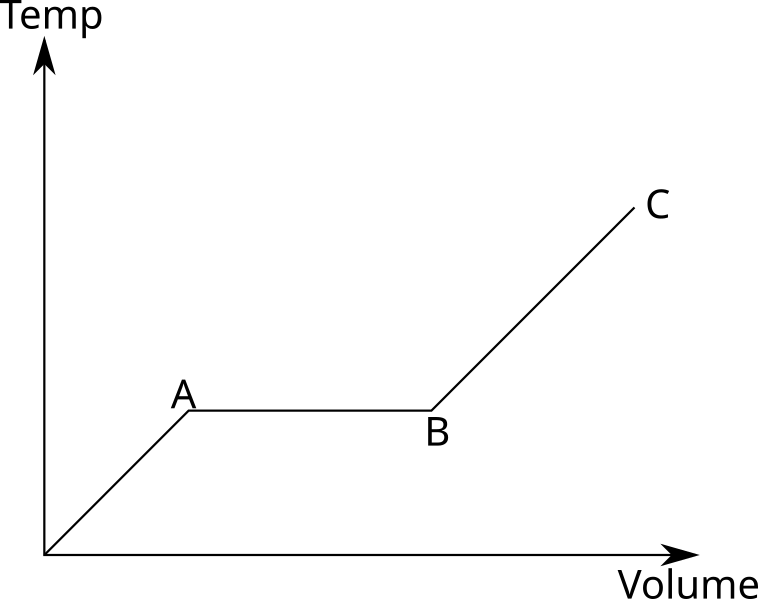
\includegraphics[scale=0.65]{./Phase_Change_Graph.png}
  \caption{Phase Change Graph}
  \label{fig:Phase_Change}
\end{figure}

The line drawn in \Cref{fig:Phase_Change} assumes that the material undergoing the phase change is under \nameref{def:Isobaric} conditions, meaning the pressure is \textbf{not} changing.
However, different pressures (under their own \nameref{def:Isobaric} conditions) will yield different, but similarly shaped, lines as well.

\begin{remark*}
  \Cref{fig:Phase_Change} is also \textbf{NOT} drawn to proportion, as the angle on the first portion of the line is typically \textbf{very} sharp.
  Obviously, \Cref{fig:Phase_Change} is an idealized graph for the temperature-volume graph of a substance and its respective phase change.
  Even though the graph is idealized, it is fine for our needs, and for most needs in \nameref{def:Thermodynamics}.
\end{remark*}

There are several notable points on the graph in \Cref{fig:Phase_Change}:
\begin{enumerate}[noitemsep]
\item Between the origin and point $A$, the substance is called a \nameref{def:Compressed_Liquid}.
  Table A.7 in the textbook has data points for some materials in this state, but the actual values vary very little.
\item At point $A$, the solid begins to boil, becoming a \nameref{def:Saturated_Liquid}, and is denoted $\SaturatedFluidVol$.
\item Between points $A$ and $B$, the substance is called a \nameref{def:Saturated_Mixture}.
  Here, there are parts of the substance in the liquid phase and the other parts of the substance are in the vapor phase.
  In the textbook, Tables A.4 and A.5 are used here.
\item At point $C$, we have a \nameref{def:Saturated_Vapor} and is denoted $\SaturatedVaporVol$.
  Table A.6 in the textbook contains data points for these vapors.
\end{enumerate}

\begin{definition}[Compressed Liquid]\label{def:Compressed_Liquid}
  A \emph{compressed liquid} is a substance, in its liquid state, as it is being heated and gaining volume, until right before it starts to boil.
  Table A.7 in the textbook has data points for some materials in this state, but the actual values vary very little.
  This is because \nameref{def:Pressure} does not change volume much.
  However, temperature \textbf{does} change the volume, therefore, treat compressed liquids as \nameref{def:Saturated_Liquid} at temperature $\Temp$, so use Table A.4.
\end{definition}

\begin{definition}[Saturated Liquid]\label{def:Saturated_Liquid}
  A \emph{saturated liquid} is a substance, starting its \nameref{def:Phase_Change} state between liquid and gas.
  The point where the liquid begins to boil is denoted $\SaturatedFluidVol$.
\end{definition}

\begin{definition}[Saturated Mixture]\label{def:Saturated_Mixture}
  A \emph{saturated mixture} is a substance in the middle of its \nameref{def:Phase_Change} state betwen a liquid and a gas.
  Parts of the substance in the liquid phase and the other parts of the substance are in the vapor phase.
  In the textbook, Tables A.4 and A.5 are used here.
\end{definition}

\begin{definition}[Saturated Vapor]\label{def:Saturated_Vapor}
  A \emph{saturated vapor} is a substance that has undergone a complete \nameref{def:Phase_Change} to fully become a gas.
  The point where this occurs is denoted $\SaturatedVaporVol$.
  Table A.6 in the textbook contains data points for these vapors.
\end{definition}

\Cref{fig:Phase_Change} can be overlayed with a curve that intersets the different isobars of that \nameref{def:Pure_Substance} based on their \nameref{def:Saturated_Liquid} and \nameref{def:Saturated_Vapor} points.

\begin{figure}[h!tbp]
  \centering
  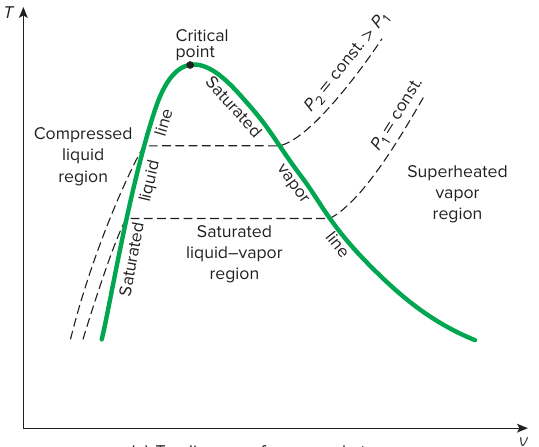
\includegraphics[scale=0.75]{./Temperature_Volume_Diagram.png}
  \caption{Temperature-Volume ($\Temp$-$\Volume$) Diagram}
  \label{fig:Temperature_Pressure_Diagram}
\end{figure}

\begin{figure}[h!tbp]
  \centering
  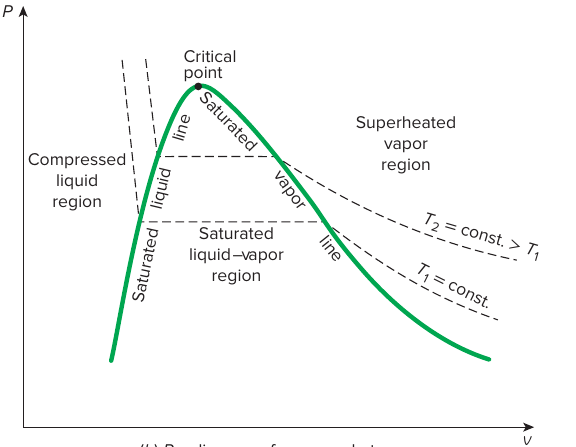
\includegraphics[scale=0.75]{./Pressure_Volume_Diagram.png}
  \caption{Pressure-Volume ($\Pressure$-$\Volume$) Diagram}
  \label{fig:Pressure_Volume_Diagram}
\end{figure}


\begin{example}{Properties of Water}
  Given water at temperature $\Temp = \SI{75}{\degreeCelsius}$ and a pressure $\Pressure = \SI{100}{\kilo\pascal}$.
  What is the water's current state?
  \tcblower{}
  We can start by looking in Table A.4 in the textbook.

  At \SI{75}{\degreeCelsius}, water boils at \SI{38}{\kilo\pascal}.
  This water will \textbf{not} boil at that temperature and pressure.
  Now going to Table A.5, which says that at our pressure, water boils at \SI{99.61}{\degreeCelsius}.

  This means that the water is in its liquid state, and is not in its \nameref{def:Saturated_Mixture} state yet.
\end{example}

\begin{example}[Problem 4.23]{What's My State}
  Given certain intensive properties of the \nameref{def:Pure_Substance}, water, fill in the table?
  \begin{enumerate}[noitemsep]
  \item $\Temp = \SI{50}{\degreeCelsius}$ and a volume of $\Volume = \SI{4.16}{\meter\cubed\per\kilo\gram}$.
  \item $\Pressure = \SI{200}{\kilo\pascal}$ and the water is in the \nameref{def:Saturated_Vapor} phase.
  \item $\Temp = \SI{250}{\degreeCelsius}$, $\Pressure = \SI{400}{\kilo\pascal}$, and $\Volume = \SI{0.595}{\meter\cubed\per\kilo\gram}$.
  \item $\Temp = \SI{110}{\degreeCelsius}$, $\Pressure = \SI{600}{\kilo\pascal}$.
  \end{enumerate}
  \tcblower{}
  \begin{center}
    \begin{tabular}{ccccc}
      \toprule
      & Temperature $\si{\degreeCelsius}$ & Pressure $\si{\kilo\pascal}$ & Volume $\si{\meter\cubed\per\kilo\gram}$ & Phase \\
      \midrule
      1 & 50 & 12.352 & 4.16 & Mixture \\
      2 & 120.21 & 200 & 0.88578 & \nameref{def:Saturated_Vapor} \\
      3 & 250 & 400 & 0.595 & Superheated Vapor/Steam \\
      4 & 110 & 600 & 0.001052 & \nameref{def:Compressed_Liquid} \\
      \bottomrule
    \end{tabular}
  \end{center}

  \begin{enumerate}[noitemsep]
  \item Phase 1:
    \begin{enumerate}[noitemsep]
    \item We need to look at Table A.4 for phase 1's saturated pressure, and find it $\SaturatedPressure$.
    \item Now, looking at the values of $\SaturatedFluidVol$ and $\SaturatedVaporVol$ for water at $\Temp = \SI{50}{\degreeCelsius}$, we see the value we're given is somewhere between those.
      Thus, this is a mixture of a \nameref{def:Saturated_Liquid} and a \nameref{def:Saturated_Vapor}.
    \end{enumerate}
  \item Phase 2:
    \begin{enumerate}[noitemsep]
    \item We were told a pressure, so we should use Table A.5.
    \item Look in Table A.5 and find $\Pressure = \SI{200}{\kilo\pascal}$, and get the saturation temperature, $\SaturatedTemp$.
    \item They told us it was a \nameref{def:Saturated_Vapor}, so we know the value is somewhere on the saturated vapor line, meaning the volume is the same as $\SaturatedVaporVol$.
    \end{enumerate}
  \item Phase 3:
    \begin{enumerate}[noitemsep]
    \item Because we are given both pressure and temperature, either Table A.4 or Table A.5 is applicable.
    \item However, neither table seems to make much sense, as on the temperature table, the pressure is too low, and on the pressure table, the temperature is too low.
    \item On both tables, our volume is significantly greater than even the $\SaturatedVaporVol$.
    \item Because $\Volume > \SaturatedVaporVol$, we go to Table A.6 for superheated water.
    \item Using Table A.6, we see that $\SaturatedVaporVol$ in the table matches the volume given to us.
    \item This means the water is now in its superheated vapor phase.
    \end{enumerate}
  \item Phase 4:
    \begin{enumerate}[noitemsep]
    \item You can start by using Table A.4 or Table A.5, but I will start with Table A.4.
    \item Find \SI{110}{\degreeCelsius} in the table.
    \item Once there, you'll notice their $\SaturatedPressure$ is \textbf{much} lower than what we were given, so we move to the next table.
    \item So, we move to Table A.5, and the temperature in the table is lower than what we were given, so we move onto the next table.
    \item This means that the temperature is lower than is needed to start boiling the water at \SI{600}{\kilo\pascal} and the pressure is too high for the water to start boiling at \SI{110}{\degreeCelsius}.
    \item This means that it must be a \nameref{def:Compressed_Liquid}.
    \item But, we said to treat \nameref{def:Compressed_Liquid}s as \nameref{def:Saturated_Liquid} at temperature $\Temp$, so use Table A.4 instead.
    \end{enumerate}
  \end{enumerate}
\end{example}

%%% Local Variables:
%%% mode: latex
%%% TeX-master: "../MMAE_320-Thermo-Reference_Sheet"
%%% End:
